% Backup D2: the Schmidt decomposition as a picture, after slides 22-23 of the
% "Journal Qlub: Intro to TNs" talk. Three steps, top to bottom:
%   (1) cut the chain in two, A | B;
%   (2) group the legs on each side -> the state IS one matrix across the cut;
%   (3) SVD that matrix -> U, the singular values, V^dagger.
% Circles = state tensors, matching the main deck; the fat lines are grouped
% (composite) indices.
\documentclass[tikz,border=3pt]{standalone}
\usepackage{amsmath,amssymb}
\usetikzlibrary{arrows.meta}
\definecolor{tnbulk}{RGB}{86,196,229}
\definecolor{tnU}{RGB}{243,180,150}
\definecolor{tnS}{RGB}{243,116,63}
\definecolor{ink}{RGB}{35,44,58}
\definecolor{warn}{RGB}{176,58,46}
\definecolor{jwnn}{RGB}{40,80,150}
\begin{document}
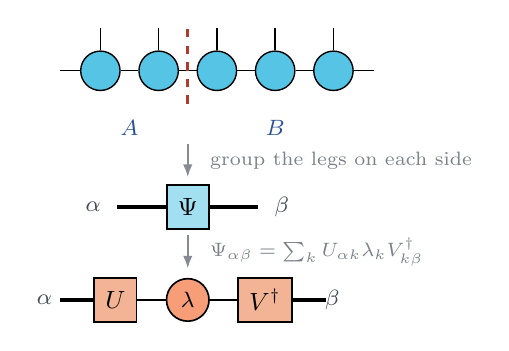
\begin{tikzpicture}[
    W/.style={circle, draw=black, fill=tnbulk, line width=0.5pt,
              minimum size=5.0mm, inner sep=0pt},
    box/.style={rectangle, draw=black, line width=0.6pt, minimum height=5.6mm,
              inner xsep=4pt, font=\small},
    sval/.style={circle, draw=black, fill=tnS!70, line width=0.6pt,
              minimum size=5.4mm, inner sep=0pt, font=\footnotesize},
    leg/.style={draw=black, line width=0.5pt},
    fat/.style={draw=black, line width=1.5pt},
    lab/.style={font=\footnotesize, color=ink!85},
    capt/.style={font=\scriptsize, color=ink!60},
    arr/.style={-{Latex[length=1.6mm]}, draw=ink!55, line width=0.7pt}]
  \def\dx{0.74}

  % ---------- (1) cut the chain -------------------------------------------
  \foreach \i in {0,...,4} { \node[W] (a\i) at ({\i*\dx},2.45) {}; }
  \foreach \i/\j in {0/1,1/2,2/3,3/4} { \draw[leg] (a\i.east) -- (a\j.west); }
  \draw[leg] (a0.west) -- ++(-0.26,0);  \draw[leg] (a4.east) -- ++(0.26,0);
  \foreach \i in {0,...,4} { \draw[leg] (a\i.north) -- ++(0,0.28); }
  \draw[warn, dashed, line width=1.0pt] ({1.5*\dx},2.98) -- ({1.5*\dx},1.95);
  \node[lab, color=jwnn] at ({0.5*\dx},1.72) {$A$};
  \node[lab, color=jwnn] at ({3.0*\dx},1.72) {$B$};

  % ---------- (2) group the legs: one matrix across the cut ---------------
  \draw[arr] ({1.5*\dx},1.52) -- ({1.5*\dx},1.10);
  \node[capt, anchor=west] at ({1.5*\dx+0.16},1.31) {group the legs on each side};

  \node[box, fill=tnbulk!55] (psi) at ({1.5*\dx},0.72) {$\Psi$};
  \draw[fat] (psi.west) -- ++(-0.62,0);
  \draw[fat] (psi.east) -- ++(0.62,0);
  \node[lab, anchor=east] at ({1.5*\dx-0.98},0.72) {$\alpha$};
  \node[lab, anchor=west] at ({1.5*\dx+0.98},0.72) {$\beta$};

  % ---------- (3) the SVD --------------------------------------------------
  \draw[arr] ({1.5*\dx},0.36) -- ({1.5*\dx},-0.06);
  \node[capt, anchor=west] at ({1.5*\dx+0.16},0.15)
    {$\Psi_{\alpha\beta}=\sum_k U_{\alpha k}\lambda_k V^{\dagger}_{k\beta}$};

  \node[sval] (sv) at ({1.5*\dx},-0.46) {$\lambda$};
  \node[box, fill=tnU] (u)  at ({1.5*\dx-0.92},-0.46) {$U$};
  \node[box, fill=tnU] (vd) at ({1.5*\dx+0.98},-0.46) {$V^{\dagger}$};
  \draw[leg] (u.east) -- (sv.west);
  \draw[leg] (sv.east) -- (vd.west);
  \draw[fat] (u.west) -- ++(-0.42,0);
  \draw[fat] (vd.east) -- ++(0.42,0);
  \node[lab, anchor=east] at ({1.5*\dx-1.60},-0.46) {$\alpha$};
  \node[lab, anchor=west] at ({1.5*\dx+1.62},-0.46) {$\beta$};
\end{tikzpicture}
\end{document}
